\documentclass[titlepage = firstcover]{scrartcl}
\usepackage[aux]{rerunfilecheck}
\usepackage{fontspec}
\usepackage[main=ngerman, english, french]{babel}

% mehr Pakete hier
\usepackage{expl3}
\usepackage{xparse}

%Mathematik------------------------------------------------------
\usepackage{amsmath}   % unverzichtbare Mathe-Befehle
\usepackage{amssymb}   % viele Mathe-Symbole
\usepackage{mathtools} % Erweiterungen für amsmath
\usepackage[
  math-style=ISO,    % \
  bold-style=ISO,    % |
  sans-style=italic, % | ISO-Standard folgen
  nabla=upright,     % |
  partial=upright,   % /
]{unicode-math}% "Does exactly what it says on the tin."
\usepackage[section, below]{placeins}

% Laden von OTF-Mathefonts
% Ermöglich Unicode Eingabe von Zeichen: α statt \alpha

\setmathfont{Latin Modern Math}
%\setmathfont{Tex Gyre Pagella Math} % alternativ zu Latin Modern Math
\setmathfont{XITS Math}[range={scr, bfscr}]
\setmathfont{XITS Math}[range={cal, bfcal}, StylisticSet=1]

\AtBeginDocument{ % wird bei \begin{document}
  % werden sonst wieder von unicode-math überschrieben
  \RenewDocumentCommand \Re {} {\operatorname{Re}}
  \RenewDocumentCommand \Im {} {\operatorname{Im}}
}
\usepackage{mleftright}
\setlength{\delimitershortfall}{-1sp}

%Sprache----------------------------------------------------------
\usepackage{microtype}
\usepackage{xfrac}
\usepackage[autostyle]{csquotes}    % babel
\usepackage[unicode, pdfusetitle]{hyperref}
\usepackage{bookmark}
\usepackage[shortcuts]{extdash}
%Einstellungen hier, z.B. Fonts
\usepackage{booktabs} % Tabellen


\title{Gedämpfte und erzwungene Schwingungen}
\author{
  David Gutnikov\\
  \href{mailto:david.gutnikov@udo.edu}{david.gutnikov@udo.edu}
 \and 
  Lasse Sternemann\\
  \href{mailto:lasse.sternemann@udo.edu}{lasse.sternemann@udo.edu}
}
\date{Durchführung am 21.01.2020}

\begin{document}
    \maketitle
    \newpage
    \tableofcontents
    \newpage

    \section{Zielsetzung}
        Der Versuch beschäfigt sich mit der genaueren Betrachtung eines LC-Schwingkreises und den ihn ihm stattfindenden Schwingungen. Dazu wird zuerst der 
        effektive Dämpfungswiderstand der gedämpften Schwingung des Schwingkreises über die Zeitabhängigkeit der Amplitude ermittelt. Zusätzlich soll auch der
        Dämpfungswiderstand ermittelt werden, der bei der Schwingung den aperiodischen Grenzfall hervorruft. Es werden auch zwei Frequenzabhängigkeiten eines 
        Serienresonanzkreises untersucht. Zum einen die Frequenzabhängigkeit der Spannung, die am Kondensator entsteht und die des Phasemunterschieds, der 
        zwischen der anregenden Spannung und der am Kondensator auftritt.
        
    \section{Theorie}
        \subsection{Gedämpfte Schwingung in einem RLC-Schwingkreis}
            In einem LC-Schwingkreis kommt es zu einer Schwingung des Stroms, wenn die Energie durch das System schwingt und entweder im Kondensator oder in
            der Spule gespeichert wird. Dabei handelt es sich um eine ungedämpfte Schwingung, da hier in der Theorie keine Energie veloren geht. In der Praxis
            hingegen geht auch in einem LC-Schwingkreis Energie über Eigenwiderstände der Bauteile verloren, sodass die Schwingung mit der Zeit an Energie 
            verliert, sofern keine neue hinzugefügt wird. Die gesamten Eigenwiderstände können als einzelner Widerstand angesehen werden, sodass nun ein 
            RLC-Schwingkreis vorliegt, in dem eine gedämpfte Schwingung ablaufen kann.
            \begin{figure}[h]
                \centering
                \caption{Das Schaltbild eines RLC-Schwingkreises. [1]}
                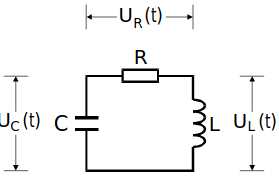
\includegraphics[width = 0.4\linewidth]{RLC.png}
                \label{fig:RLC}
            \end{figure}
            \FloatBarrier
            Um das Schwingungsverhalten des RLC-Schwingkreises mathematisch beschreiben zu können, müssen die Abhängigkeiten der Spannungen betrachtet werden.
            Diese Betrachtung liefet über die Kirchhoffsche Maschenregel folgende Bedingung für die Spannungen an Widerstand, Spule und Kondensator:
            \begin{equation}
                U_{\text{R}}(t) + U_{\text{C}}(t) + U_{\text{L}}(t) = 0
                \label{eqn:Masche}
            \end{equation}  
            Durch Einsetzen der bekannten Formeln für die Spannungen an den einzelnen Bauteilen und der Definition des Stroms,
            \begin{align}
                U_{\text{R}}(t) = R \cdot I(t) &\qquad U_{\text{C}}(t) = \frac{Q(t)}{C} & U_{\text{L}}(t) = L \cdot \dot{I} &\qquad I = \dot{Q} 
                \label{eqn:Spannungen}
            \end{align}
            ergibt sich die Differentialgleichung für die gedämpfte Schwingung.
            \begin{equation}
                \ddot{I} + \frac{R}{L} \dot{I} + \frac{1}{LC} \cdot I = 0
            \end{equation}
            Das Lösen dieser Differentialgleichung über den Schwingungsansatz
            \begin{equation*}
                I(t) = e^{i\omega t}
            \end{equation*} 
            ergibt folgende Formel für die Schwingfrequenz $\omega$:
            \begin{equation}
                \omega_{\text{1,2}} = i\frac{R}{2L} \pm \sqrt{\frac{1}{LC} + \frac{R^2}{4L^2}}
                \label{eqn:omega}
            \end{equation}
            Da die Wurzel zu zwei unterschiedlichen Frequenzen führt, wird die Lösung der Differentialgleichung durch eine Kombination von E-Funktionen
            beschrieben.
            \begin{align}
                &I(t) = A_1 \cdot e^{i\omega_1 t} + A_2 \cdot e^{i \omega_2 t} \\
                &\text{wird mit} \qquad 2\pi\mu := \frac{R}{2L} \qquad \text{und} \qquad 2\pi\nu ' := \sqrt{\frac{1}{LC}-\frac{R²}{4L²}} \\
                &\text{zu} \qquad I(t) = e^{2\pi\mu t} \cdot (A_1 \cdot e^{i2\pi\nu t} + A_2 \cdot e^{-i2\pi\nu t})
                \label{eqn:DGlösung}
            \end{align}
            Dabei müssen 3 Fälle für den Wurzelterm betrachtet werden. Der erste liegt darin, dass der Term innerhalb der Wurel positiv und diese 
            dementsprechend reell ist. In diesem Fall lässt sich die Formel für den Strom \ref{eqn:DGlösung} umschreiben zu:
            \begin{equation}
                I(t) = A_0 \cdot e^{-i2\pi\nu t} \cdot \text{cos}(2\pi\nu t + \eta)
            \end{equation}
            Dies beschreibt eine gedämpfte Schwingung mit der Schwingungsdauer $T$ und der Abklingzeit $T_{\text{ex}}$.
            \begin{equation}
                T = \frac{2\pi}{\sqrt{\frac{1}{LC}-\frac{R²}{4L²}}} \qquad T_{\text{ex}} = \frac{\text{2L}}{\text{R}}
                \label{eqn:Tpositiv}
            \end{equation}
            Der zweite Fall liegt vor, wenn der Term in der Wurzel negativ und diese imaginär ist. In diesem Fall ist in der Formel für den Strom kein 
            schwingungserzeugender Teil mehr und der Strom,
            \begin{equation}
                I(t) \propto e^{-\left(\frac{\text{R}}{\text{2l}}-\sqrt{\frac{\text{R²}}{\text{4L²}}-\frac{1}{\text{LC}}}\right)\cdot t} ,
                \label{eqn:Dämpffall}
            \end{equation}
            geht, wie in Abbildung \ref{fig:RDämpfungLC} zu sehen, mit der Zeit gegen 0. Dies wird Kriechfall genannt.
            \begin{figure}[h]
                \centering
                \caption{Mögliche Stromverläufe für den Kriechfall einer gedämpften Schwingung. Die schwarze gestrichelte Linie beschreibt den aperiodischen Grenzfall. [1]}
                \includegraphics[width = 0.4\linewidth]{Dämpffall.png}
                \label{fig:RDämpfungLC}
            \end{figure}
            \FloatBarrier
            Der letzte zu betrachtende Fall liegt beim verschwinden der Wurzel vor, also wenn
            \begin{equation*}
                \frac{1}{\text{LC}} = \frac{\text{R²}}{\text{4L²}}
            \end{equation*}
            gilt. Dann lässt sich der Strom wie folgt darstellen
            \begin{equation}
                I(t) = A \cdot e^{-\frac{\text{R}}{\text{2L}}\text{t}} = A \cdot e^{-\frac{\text{t}}{\sqrt{\text{LC}}}}.
                \label{eqn:aperio}
            \end{equation}
            Dabei fällt der Strom schneller als bei allen anderen Kriechfällen und hat auch keinen Nulldurchgang. Dieser Einzelfall ist in der 
            technischen Anwendung besonders wichtig und heißt aperiodischer Grenzfall.

        \subsection{Erzwungene Schwingungen in einem RLC-Schwingkreis}
            Das Verhalten eines von außen, periodisch angeregten Schwingkreises kann durch die Ansteuerung des bekannten Schwingkreises durch eine externe Spannung, z.B.
            über einen Sinusgenerator \ref{figangeregt}, untersucht werden. 
            \begin{figure}[h]
                \centering
                \caption{Das Schaltbild des durch einen Sinusgenerator angeregten RLC-Schwingkreises. [1]}
                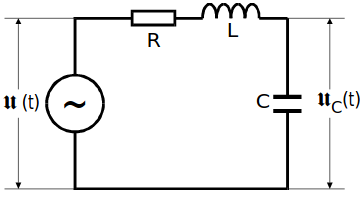
\includegraphics[width = 0.4\linewidth]{angeregt.png}
                \label{fig:angeregt}
            \end{figure}
            \FloatBarrier
            Die äußere Anregung erzeugt eine Inhomogenität in der zugehörigen Differentialgleichung.
            \begin{equation}
                \text{LC}\ddot{U}_{\text{C}}(t) + \text{RC} \dot{U_{\text{C}}(t)} + U_{\text{C}}(t) = U_0 \cdot e^{i\omega t}
                \label{eqn:angeregt}
            \end{equation}
            Diese Gleichung lässt sich nach 
            \begin{equation*}
                U(\omega) \quad \text{mit} \quad U_\text{C}(\omega,t) = U(\omega) \cdot e^{i\omega t}
            \end{equation*}
            auflösen:
            \begin{equation}
                U(t) = \frac{U_0 (1-\text{LC}\omega^2-i\omega \text{RC})}{(1-\text{LC}\omega^2)^2 + \omega^2\text{R²C²}}
                \label{eqn:Uangeregt}
            \end{equation}
            Da $U(t)$ komplex ist, hat die Spannung eine Phase, die sich durch das Verhältnis von Realteil und Imaginärteil bestimmen lässt.
            \begin{equation}
                \phi (\omega) = \text{arctan}\left(\frac{Im(U)}{Re(U)}\right) = \text{arctan}\left(\frac{-\omega \text{RC}}{1-\text{LC}\omega^2}\right)
                \label{eqn:Phase}
            \end{equation}
            Das Betrachten dieser Beziehung liefert Schlüsse auf den Zusammenhang zwischen Frequenzen und Phasenverschiebungen. So gilt,
            \begin{align}
                \phi_1 = \frac{\pi}{4}  &\qquad \omega_1 = + \frac{\text{R}}{\text{2L}} + \sqrt{\frac{\text{R²}}{4L²} + \frac{1}{\text{LC}}}, \\
                \phi_2 = \frac{3\pi}{4} &\qquad \omega_2 = - \frac{\text{R}}{\text{2L}} + \sqrt{\frac{\text{R²}}{4L²} + \frac{1}{\text{LC}}}.
                \label{eqn:freq}
            \end{align}
            Daraus kann direkt die Differenz von $\omega_1$ und $\omega_2$ abgelesen werden.
            \begin{equation}
                \omega_1 - \omega_2 = \frac{\text{R}}{\text{L}}
                \label{eqn:w1-w2}
            \end{equation}
            Der Betrag der Gleichungen $U(t)$ \ref{eqn:Uangeregt} und $U_{\text{C}}$ muss gleich sein, sodass man nun die gewünschte Frequenzabhängigkeit
            der Resonanzspannung $U_{\text{C}}$ angeben kann:
            \begin{equation}
                U_{\text{C}}(\omega) = \frac{U_0}{\sqrt{\left(1-\text{LC}\omega^2\right)^2 + \omega^2\text{R²C²}}}
                \label{eqn:Uvonw}
            \end{equation}  
            Eine Untersuchung des Grenzverhaltens der Gleichung zeigt, dass die Spanung $U_{\text{C}}$ für gegen $\infty$ gehende Frequenzen gegen Null und für
            gegen Null gehende Frequenzen gegen die Erregerspannung $U_0$ geht. Eine ganz besondere Frequenz ist die Resonanzfrequenz,
            \begin{equation}
                \omega_{\text{Res}} = \sqrt{\frac{1}{\text{LC}}-\frac{\text{R²}}{\text{2L²}}},
                \label{eqn:Resonanzfreq}
            \end{equation}
            bei der die Resonanz eintritt und die Spannung $U_{\text{C}}$ sogar die Erregerspannung $U_0$ übersteigt und gegen einen Maximalwert läuft.
            Wenn sich die Subtrahenten in der Wurzel wiefolgt verhalten,
            \begin{equation*}
                \frac{\text{R²}}{\text{2L²}} << \frac{1}{\text{LC}}
            \end{equation*} 
            läuft die Resonanzfrequenz gegen die Frequenz des unangeregten Schwingkreises
            \begin{equation*}
                \omega_0^2 = \frac{1}{\text{LC}}
            \end{equation*}
            und die Spannung $U_{\text{C}}$ nimmt das $q$-fache der Erregerspannung $U_0$ an.
            $q$ beschreibt dabei die Güte des Schwingkreises und ist definiert als:
            \begin{equation}
                q = \frac{1}{\omega_0 \text{RC}}
                \label{eqn:Güte}
            \end{equation}
            Ähnlich der Güte beschreibt auch die Breite der durch $U_{\text{C}}$ beschriebenen Resonanzkurve die Qualität des Systems und der Resonanz. 
            Die Breite lässt sich durch die Frequenzen $\omega_+$ und $\omega_-$ bestimmen. Dies rührt aus der Gleichung
            \begin{align*}
                \frac{U_0}{\sqrt{2}} \cdot \frac{1}{\omega_0\text{RC}} = \frac{U_0}{\text{C}\cdot \sqrt{\omega_{\pm}^2\text{R²} + \left(\omega_{\pm}^2\text{L}-\frac{1}{\text{C}}\right)^2}} \\
                \text{und der Tatsache} \qquad \frac{\text{R²}}{L²} << \omega_0^2,
            \end{align*} 
            sodass sich für die Breite
            \begin{equation}
                \omega_+ - \omega_- \propto \frac{\text{R}}{\text{L}}
                \label{eqn:breiteResonanzkurve}
            \end{equation}
            ergibt. Diese gleicht nun im Fall einer Schwachen Dämpfung der Differenz von $\omega_1$ und $\omega_2$ \ref{eqn:w1-w2}.

    \section{Durchführung}
        \subsection{Frequenzabhängigkeit der Amplitude bei einer gedämpften Schwingung}
            Zunächst soll der effektive Dämpfungswiderstand des Schwingkreises bestimmt werden. Dazu wird die in Abbildung xxx zu sehende Schaltung verwendet.
            Jedoch wird kein Nadelimpuls, sondern eine Rechtecksspannung angelegt. Die entstehende gedämpfte Schwingung kann auf dem Oszilloskop beobachtet 
            werden. Zur Bestimmung des Dämpfungswiderstands muss die Abhängigkeit der Amplitude von der Zeit ermittelt werden. Dazu wird der zeitliche Abstand
            zwischen Extrema der Schwingung am Oszilloskop abgelesen.
            \begin{figure}[h]
                \centering
                \caption{Das Schaltbild zur Messung der Zeitabhängigkeit der Amplitude einer gedämpften Schwingung. Der Nadelimpuls wird jedoch durch eine Rechtecksspannung ersetzt. [1]}
                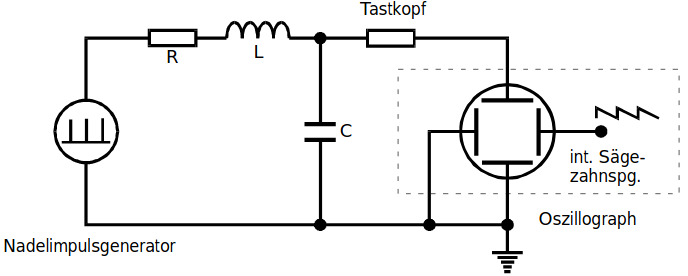
\includegraphics[width = 0.4\linewidth]{MessungA.png}
                \label{fig:MessungA}
              \end{figure}
              \FloatBarrier

        \subsection{Bestimmung des Dämpfungswiderstands beim aperiodischen Grenzfall}
            Nun soll der Dämpfungswiderstand ermittelt werden, bei dem der aperiodische Grenzfall eintritt. Dieser liegt, wie bereits erklärt vor, wenn der
            Strom ohne Nulldurchgang, auch Überschwingung genannt, gegen Null geht. Dazu wird an sich dieselbe Schaltung wie zuvor genutzt, jedoch der 
            Widerstand durch einen variablen Widerstand ersetzt, der zunächst auf seinen maximalen Wert eingestellt ist. Nun wird dieser Widerstand verringer
            bis oben beschriebenes Verhalten eintritt und der Dämpfungswiderstand des aperiodischen Grenzfalls so gefunden wurde.
            \begin{figure}[h]
                \centering
                \caption{Das Schaltbild zur Messung des Dämpfungswiderstands beim aperiodischen Grenzfall. Der Nadelimpuls wird wieder durch eine Rechtecksspannung ersetzt. [1]}
                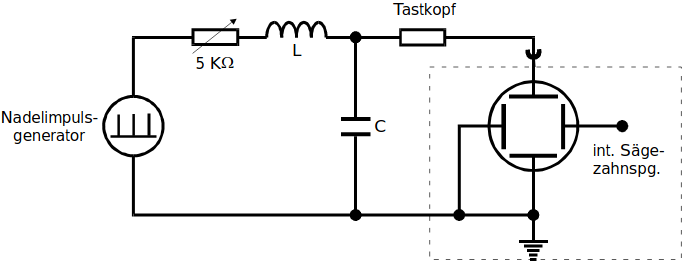
\includegraphics[width = 0.4\linewidth]{MessungB.png}
                \label{fig:MessungB}
              \end{figure}
              \FloatBarrier

        \subsection{Frequenzabhängigkeit der Kondensatorspannung in einem Serienresonanzkreis}
              Zur Bestimmung der Frequenzabhängigkeit der Kondensatorspannung eines Serienresonanzkreises wird zunächst Schaltung \ref{fig:MessungC} aufgebaut und die Erregerspannung in Abhängigkeit der Frequenz gemessen werden. Nachdem dies geschehen ist, wird nun ganz simpel die Anregungsfrequenz variiert und gleichzeitig die Kondensatorspannung abgelesen. Dies geschieht um den Bereich der Resonanzfrequenz in kleineren Intervallen, da dieser Bereich einer genaueren Betrachtung unterzogen werden soll. Die bereits gemessene Erregerspannung wird nun benötigt, da sie womöglich nicht konstant ist. Daher wird der Quotient aus Kondensatorspannung und Erregerspannung gebildet. 
              \begin{figure}[h]
                \centering
                \caption{Das Schaltbild zur Messung der Frequenzabhängigkeit der Kondensatorspannung eines Serienresonanzkreises. [1]}
                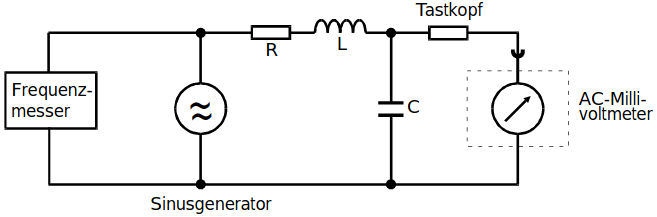
\includegraphics[width = 0.4\linewidth]{MessungC.png}
                \label{fig:MessungC}
              \end{figure}
              \FloatBarrier

        \subsection{Frequenzabhängigkeit der Phase zwischen Erregerspannung und Kondensatorspannung in einem Serienresonanzkreis}
            Um die Frequenzabhängigkeit der Phase zwischen Erregerspannung und Kondensatorspannung in einem Serienresonanzkreis zu ermitteln, werden beide 
            Spannungen, wie in Abbildung \ref{figMessungD} zu sehen, an ein Oszilloskop angeschlossen und dieses dann im XX-Betrieb verwendet. So lässt sich der Phasenunterschied der beiden Spannungen leicht ermitteln, indem der Abstand zwischen den Nulldurchgängen der beiden Spannungen am Oszilloskop
            abgelesen wird.
            \begin{figure}[h]
                \centering
                \caption{Das Schaltbild zur Messung der Frequenzabhängigkeit der Phase zwischen Kondensatorspannung und Erregerspannung eines Serienresonanzkreises. [1]}
                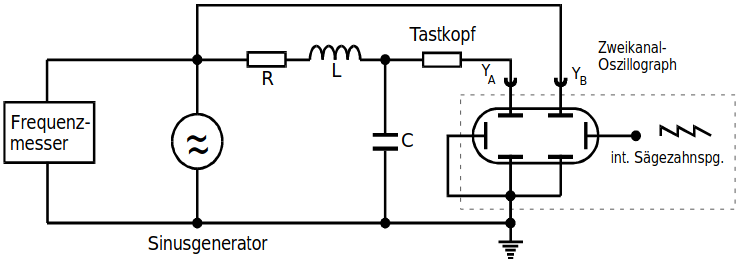
\includegraphics[width = 0.4\linewidth]{MessungD.png}
                \label{fig:MessungD}
              \end{figure}
              \FloatBarrier

    \section{Auswertung}
        Die notierten Werte sind
        \begin{align}
            L &= (10,11 \pm 0,03) \text{mH} \\
            C &= (2,093 \pm 0,003) \text{nF} \\
            R_1 &= (48,1 \pm 0,1) \Omega \\
            R_2 &= (509,5 \pm 0,5) \Omega
        \end{align}
        Diese Werte sind die Kenngrößen des Schwingkreises und werden in weiteren Rechnungen verwendet.
        \subsection{Frequenzabhängigkeit der Spannungsamplitude}
            Es wird die Zeitabhängigkeit der Spannungsamplitude untersucht. Dazu wird der Verlauf der Amplitude mit einer Thoeriekurve verglichen.
            \begin{table}[h]
                \centering
                \caption{Die Werte der Amplituden in einer Schwingung.}
                \label{tab:Tabelle1}
                \begin{tabular}{c c}
                    \toprule
                    {$t / \mu\text{s}$} & {$U_\text{Amplitude} / \text{mV}$}\\
                    \midrule
                    0  &  145 \\ 
                    16 & -140 \\
                    28 &  122 \\ 
                    44 & -117 \\
                    58 &  104 \\ 
                    73 & -100 \\
                    87 &  88  \\
                    102 & -82 \\
                    118 & 74  \\
                    133 & -71 \\
                    147 & 62  \\
                    163 & -60 \\
                    178 & 52  \\
                    195 & -50 \\
                    211 & 44  \\
                    226 & -42 \\
                    \bottomrule
                \end{tabular}
            \end{table}
            \FloatBarrier
            \noindent
            Dabei sind die positiven Werte jeweils die Werte Spannungsmaxima und die negativen Werte sind den Spannungsminima zugehörig.
            \begin{figure}[h]
                \centering
                \caption{Die gefitteten Messwerte und die Theoriekurve zu den Messwerten aus \ref{tab:Tabelle1}.}
                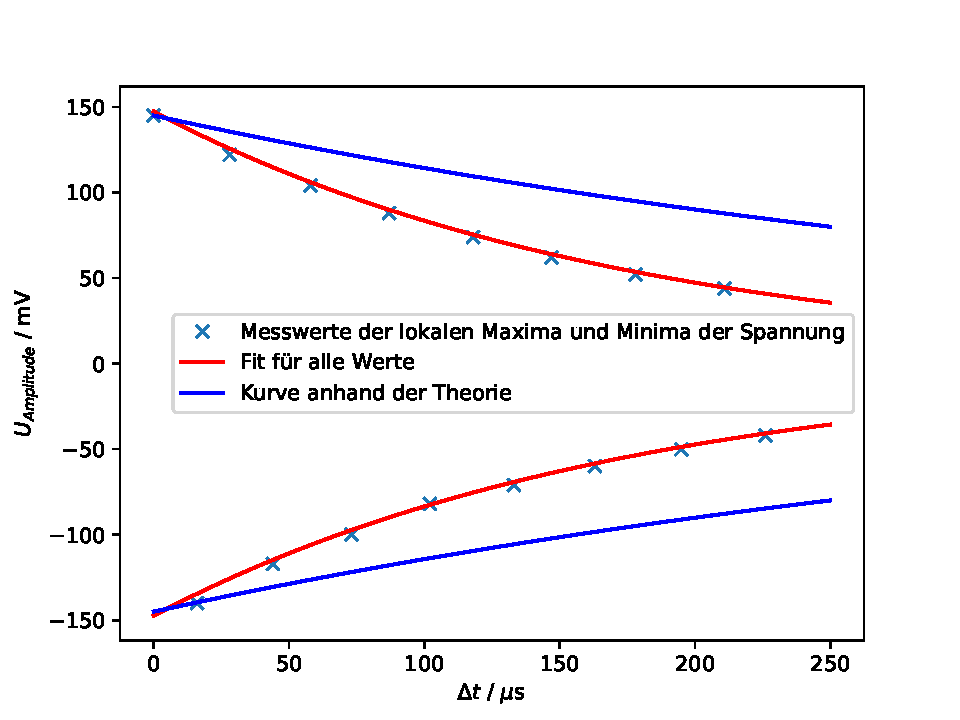
\includegraphics[width = 0.7\linewidth]{Spannungsamplituden.pdf}
                \label{fig:Spannungsamplituden}
            \end{figure}
            \FloatBarrier
            \noindent
            Aus den Parametern $A_0$ und $\mu$ der Fit-Funktion
            \begin{equation*}
                A = A_0 \cdot e^{-2 \pi \mu t}
            \end{equation*}
            werden der effektiven Dämpfungswiderstand und $R_\text{eff}$ und die Abklingzeit $T_\text{ex}$ berechnet mit \eqref{eqn:Dämpffall}:
            \begin{align}
                R_\text{eff} &= (114,8 \pm 2,4) \; \Omega \\
                T_\text{ex} &= (176 \pm 4) \; \mu \text{s}
            \end{align}
            Der Widerstand in der benutzten Schaltung $R_1 = (48,1 \pm 0,1) \Omega$ weicht um $66,7 \Omega$ von dem berechnete effektiven Dämpfungswiderstand
            ab. Das kann an dem nicht miteinbezogenen Innenwiderstand des Generators von $50 \Omega$ liegen.

        \subsection{Widerstand für aperiodischen Grenzfall}
            Wie schon in der Durchführung erläutert variiert man den Dämpfungswiderstand in der Schaltung bis es gerade keinen Nulldurchgang der Spannung gibt.
            Dieser Wert ist dann der Widerstand für den der aperiodische Grenzfall vorliegt.
            \begin{equation*}
                R_\text{ap} = 3470 \; \Omega
            \end{equation*}
            Mit
            \begin{equation*}
                \frac{R_\text{ap}²}{2L²} = \frac{1}{LC}
            \end{equation*} 
            berechnet man den Theoriewert des Widerstandes welcher bei
            \begin{equation*}
                R_{ap_t} = 4396 \; \Omega
            \end{equation*}
            liegt.
            Es wird die Abweichung vom Theoriewert folgendermaßen bestimmt
            \begin{equation}
                a_{R_{ap}} = \frac{|R_{ap_t} - R_\text{ap}|}{R_{ap_t}} = 21,06 \%
                \label{eqn:abweichung}
            \end{equation}
            Der Messwert scheint nicht zu weit vom Theoriewert abzuweichen. Mögliche Fehlerquellen könnten das ungenaue Ablesen und der nicht akkurat einstellbare Drehknopf des variierbaren Widerstandes sein.
            
        \subsection{Frequenzabhängigkeit der Kondensatorspannung}
            In \ref{tab:Tabelle2} stehen die Messwerte der Frequenz $f$, der Kondensatorspannung $U_\text{C}$ und der Erregerspannung $U_0$.
            \begin{table}[h]
                \centering
                \caption{Die Messwerte der Spannungen, ihrer Phase, Frequenz aufgetragen.}
                \label{tab:Tabelle2}
                \begin{tabular}{c c c c}
                    \toprule
                    {$f / \text{kHz}$} & {$U_\text{C} / \text{mV}$} & {$U_0 / \text{mV}$} & {$\varphi / \mu$s} \\
                    \midrule
                    10   &  121 & 430 & -   \\
                    15   &  134 & 430 & 1,7 \\
                    18   &  148 & 430 & 2   \\
                    20   &  162 & 425 & 2,1 \\
                    22   &  180 & 425 & 2,4 \\
                    24   &  200 & 425 & 2,7 \\
                    26   &  230 & 420 & 3   \\
                    28   &  275 & 410 & 3,5 \\
                    30   &  330 & 400 & 4,5 \\
                    32   &  390 & 395 & 6   \\
                    34   &  410 & 390 & 7,9 \\
                    36   &  350 & 395 & 9,5 \\
                    38   &  275 & 410 & 10  \\
                    40   &  215 & 415 & 10,5\\
                    42   &  170 & 420 & 10,5\\
                    44   &  145 & 420 & 10  \\
                    46   &  115 & 425 & 10  \\
                    48   &  97  & 425 & 10  \\
                    50   &  87  & 425 & 9,7 \\
                    55   &  75  & 425 & 9   \\
                    57.5 &  55  & 427 & 8,5 \\
                    \bottomrule
                \end{tabular}
            \end{table}
            \FloatBarrier
            \noindent
            Aus \ref{fig:Spannungsverhaeltnis} kann die Resonanzfrequenz bestimmt und dann mit dem Theoriewert verglichen werden.

            \begin{figure}[h]
                \centering
                \caption{Die Messwerte halblogarithmisch für das Spannungsverhältnis aus \ref{tab:Tabelle2} gegen die Frequenz aufgetragen.}
                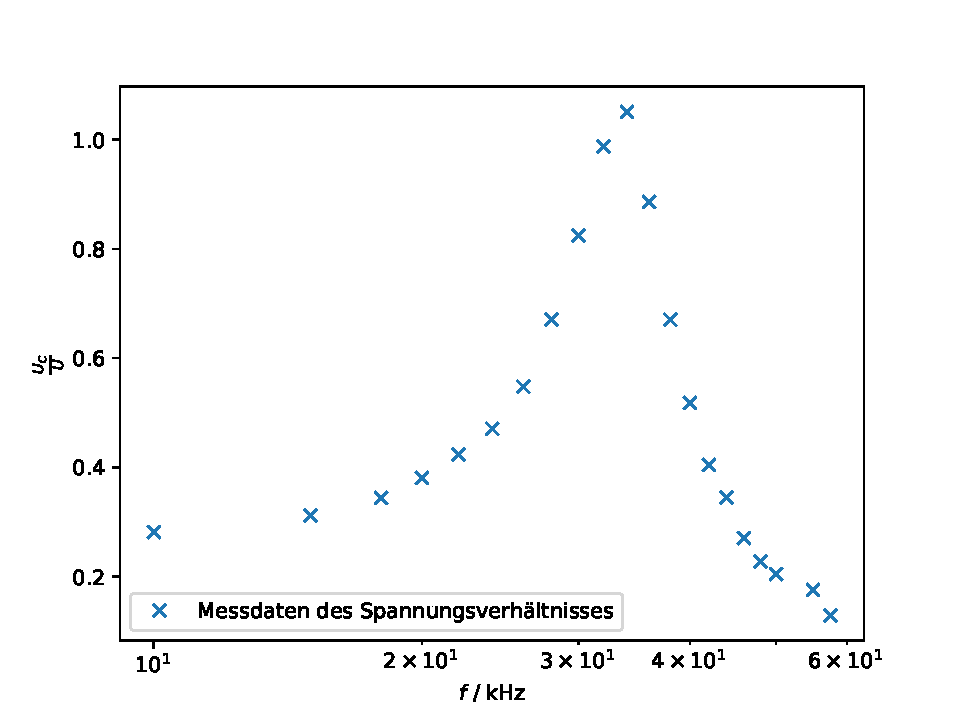
\includegraphics[width = 0.7\linewidth]{Spannungsverhaeltnis_log.pdf}
            \end{figure}
            \FloatBarrier
            \begin{figure}[h]
                \centering
                \caption{Die Messwerte linear für das Spannungsverhältnis aus \ref{tab:Tabelle2} gegen die Frequenz aufgetragen.}
                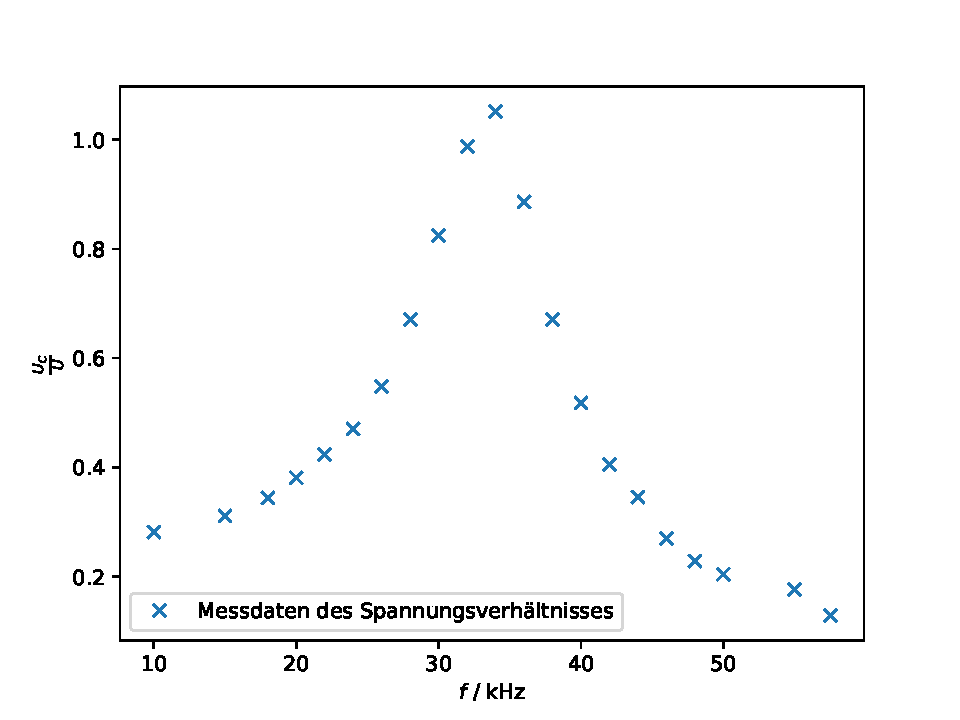
\includegraphics[width = 0.7\linewidth]{Spannungsverhaeltnis.pdf}
                \label{fig:Spannungsverhaeltnis}
            \end{figure}
            \FloatBarrier
            \noindent
            Aus \ref{fig:Spannungsverhaeltnis} ist eine Resonanzfrequenz von ca. $f_\text{res} = 35 \;$kHz ablesbar, welche analog zu \eqref{eqn:abweichung}
            mit dem Theoriewert von $f_\text{res} = 34,59 \;$kHz verglichen wird:
            \begin{equation*}
                a_{f_\text{res}} =  11,72 \%
            \end{equation*}
            Die Güte wird einfach an \ref{fig:Spannungsverhaeltnis} abgelesen und mit \eqref{eqn:Güte} wird der theoretische Wert berechnet:
            \begin{align}
                q &= 1,08 \\
                q_\text{theorie} &= 19,14 \\
                a_\text{q} &= 94,38 \%
            \end{align}
            Es scheint, dass es einen systematischen Fehler in unserer Berechnung gibt und der Theoriewert um eine Zehnerpotenz zu groß ist.
            Die theoretische Breite der Resonanzkurve wird nach \eqref{eqn:w1-w2} bestimmt und die experimentell bestimmte Breite wird aus
            \ref{fig:Spannungsverhaeltnis} abgelesen:
            \begin{align}
                \nu_1 - \nu_2 &= 9 \; \text{kHz} \\
                (\nu_1 - \nu_2)_\text{Theorie} &= 1,807 \; \text{kHz} \\
                a_{\nu} &= 398 \%                
            \end{align}
            Auch hier gibt es augenscheinlich eine sehr große Abweichung, welcher wahrscheinlich einem Fehler in der Berechnung zuzuschulden ist.

            \begin{figure}[h]
                \centering
                \caption{Die Messwerte halblogarithmisch für die Phase aus \ref{tab:Tabelle2} gegen die Frequenz aufgetragen.}
                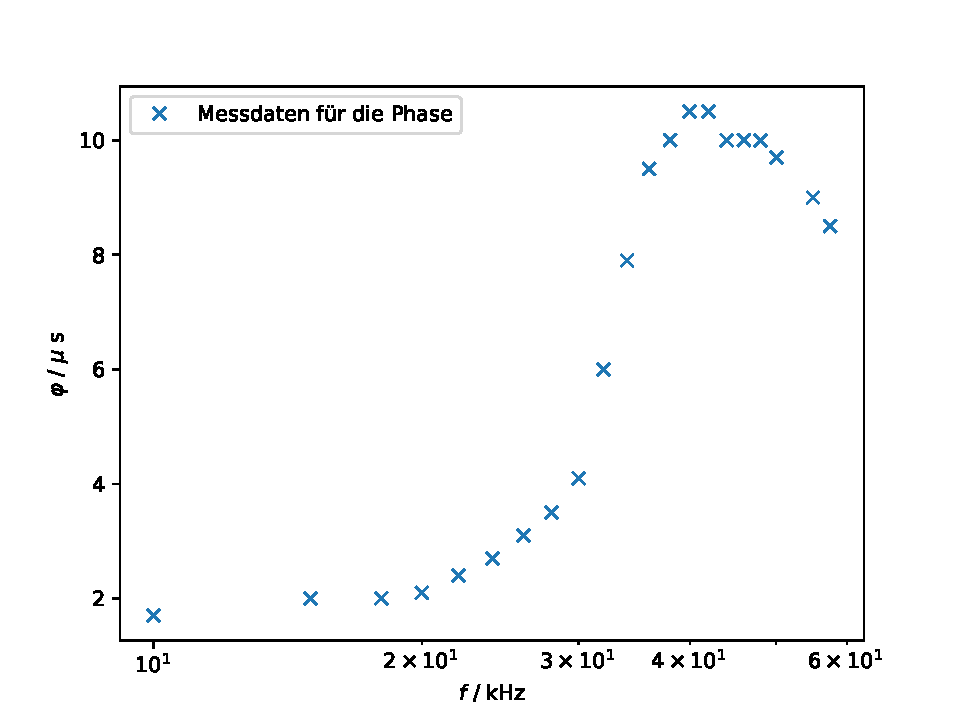
\includegraphics[width = 0.7\linewidth]{Phase_log.pdf}
            \end{figure}
            \FloatBarrier
            \begin{figure}[h]
                \centering
                \caption{Die Messwerte linear für die Phase aus \ref{tab:Tabelle2} gegen die Frequenz aufgetragen.}
                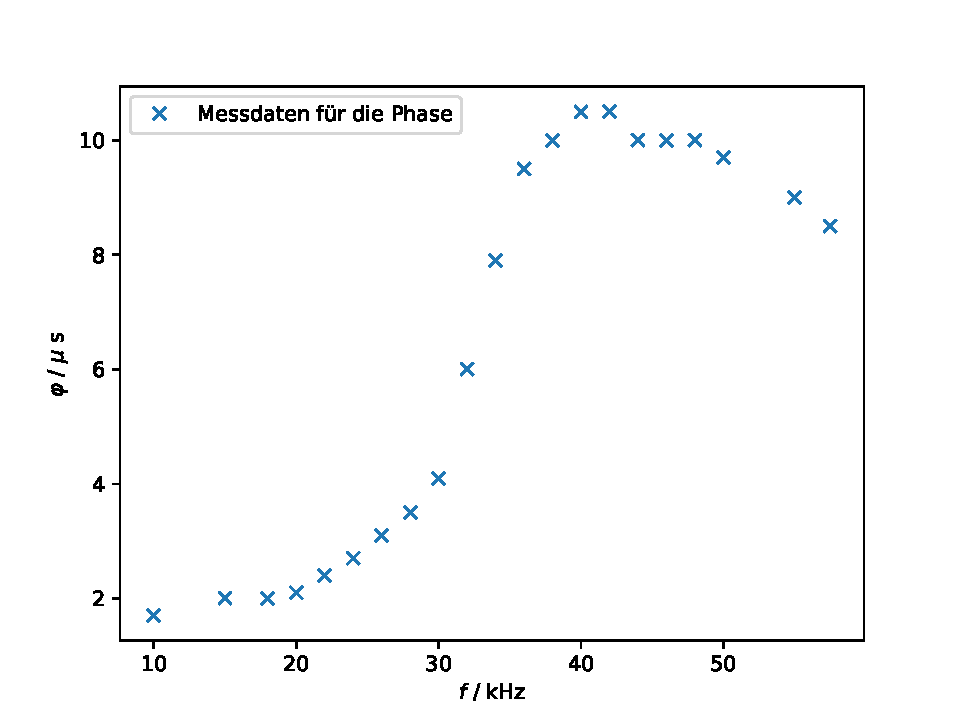
\includegraphics[width = 0.7\linewidth]{Phase.pdf}
                \label{fig:phase}
            \end{figure}
            \FloatBarrier
            \noindent
            Hier ist aus \ref{}eine Resonanzfrequenz von ca. $f_\text{res} = 34 \;$kHz abzulesen, die vom zuvor berechneten Theoriewert von
            $f_\text{res} = 34,59 \;$kHz um $a_res = 1,72 \%$ abweicht.
            Mit \eqref{eqn:omega} werden $\nu_\text{1, theo}$ und $\nu_\text{2, theo}$ berechnet. Also die Frequenzen für die die Phase zwischen
            Erregerspannung und Kondensatorspannung $\frac{\pi}{4}$ und $\frac{3\pi}{4}$ beträgt.
            \begin{align}
                \nu_\text{1, theo} &= 34.98 \; \text{kHz} \\
                \nu_\text{2, theo} &= 34.422 \; \text{kHz}
            \end{align}


        \section{Diskussion}
            Von der Form her sehen die einzelnen Graphen so aus wie es erwartet wird. Die Werte für den effektiven Dämpfungswiderstand und den Grenzwiderstand
            für den aperiodischen Grenzfall liegen im Toleranzbereich, wenn man den Innenwiderstand des Generators mit einbezieht. Doch die Werte für die
            Güte und die Breite der Resonanzkurve weichen sehr stark von ihren jeweiligen Theoriewerten ab, was möglicherweise zum Teil einem nicht so genauen
            Ablesen der Werte und einem systematischen Fehler in der Rechnung, welcher auch nach wiederholtem Prüfen nicht behoben werden konnte, zu
            verschulden ist.

    \section{Literaturverzeichnis}
        [1] \textit{Versuchsanleitung V354 - Gedämpfte und erzwungene Schwingungen.} TU Dormund, 2019
             
\end{document}